\chapter{Implementation}
This section covers the implementation of the tool, the technologies used, and the code's organization. It also outlines the tool's purpose and its target users.

\section{Purpose and Intended Audience}
The tool targets researchers and developers involved in testing self-driving vehicles. Its purpose is to streamline road creation for testing these cars, eliminating the need for users to write road generation algorithms. Instead, they can simply provide textual descriptions of the roads they want to create.


\section{Technologies}
\subsection{Python}
RoadGPT is written in Python, an \textit{"interpreted, object-oriented, high-level programming language with dynamic semantics"} \cite{python}. Python enables rapid development across different domains, from web development to data analysis and machine learning. With its extensive standard library and numerous third-party packages, it helps programmers solve complex problems efficiently \cite{python}. The main libraries used for the tool are the following:

\begin{itemize}
    \item \textbf{OpenAI}: provides easy access to the OpenAI API and is used to communicate with ChatGPT \cite{OpenAI}.
    \item \textbf{NumPy}: an open-source library used for working with numerical data in Python. It includes a wide variety of mathematical functions \cite{NumPy}.
    \item \textbf{SciPy}: a collection of mathematical algorithms and functions built on NumPy \cite{SciPy}.
    \item \textbf{BeamNGpy}: a package that provides a Python API to BeamNG.tech \cite{BeamNGpy}.
\end{itemize}

\subsection{OpenAI API}
The OpenAI API is used to enhance user road descriptions by returning more detailed descriptions in a standardized format, simplifying further processing. I selected the GPT-3.5 turbo model for this task because it supports enforced JSON responses. At the time of writing, the model is priced at \$0.0005 per 1000 tokens for inputs and \$0.0015 per 1000 tokens for outputs. Tokens represent pieces of words, with 1000 tokens approximately equaling 750 words \cite{OpenAIPricing}.

\subsection{BeamNG.tech}
BeamNG.tech has been chosen as the simulator for several reasons. Firstly, the BeamNGpy package simplifies scenario creation and data extraction for visualization. Secondly, the use of mesh roads enables the generation of 3D roads. Lastly, BeamNG.tech features a realistic physics simulation, ensuring accurate vehicle behavior and environmental interactions. Together, these attributes make BeamNG.tech a comprehensive and reliable option for simulation tasks.

%\section{Code Structure}
%Since the code is based on the SBST tool competition \cite{GambiJRZ} the code follows a similar structure. The \textbf{levels\_template/tig folder}, contains the files to create the level, alongside the textures of the roads.

%In \textbf{self\_driving} you can find the files related the simulations in BeamNG.tech. The files in this folder are used to set up and run the simulations.

%The files in the \textbf{code\_pipeline} folder 



\section{RoadGPT}
RoadGPT is a command line tool that can be called with different parameters. The code is based on the SBFT tool competition \cite{SBFT}.

\begin{itemize}
    \item \textbf{beamng-home}: The location of the BeamNG.tech executable.
    \item \textbf{beamng-user}: A directory where levels and other BeamNG-related data will be copied
    \item \textbf{model}: A parameter specifying whether to use OpenAI's assistants or the completions API. Assistants use instructions to tune their personalities and capabilities \cite{OpenAI}. Once created, users can access existing assistants by the latter's ID. Completion models take a list of messages as input and return an answer generated by the model \cite{OpenAI}. In the case of RoadGPT, these messages are just the system message, giving the model some context, ground rules, and the user's road description.
\end{itemize}

\subsection{OpenAI API Connection}
After the user provides the road description and specifies the generation budget (the number of road descriptions to be obtained from ChatGPT), RoadGPT initiates an API call using the provided parameters. This API call includes a system prompt, a prompt specified by the user, and defines the response format as JSON. The system prompt serves as the initial instruction for the model, guiding it on what to generate based on the user's input. 

The system prompt used is: 

\textit{"You are a road designer, who designs roads to test the lane keeping functionality of self driving vehicles. People give you descriptions of roads and you create more detailed descriptions of novel roads, where you split the road into segments. These descriptions are then turned into coordinates, so keep the coordinate values in mind. Since you are testing the lane keeping functionality of self driving vehicles, you want to stress it.}

\textit{Here are some ground rules:}
\begin{itemize}
    \item \textit{The roads should be diverse, that means given the same description don't create the same road (Start in different directions, etc.) }
    \item \textit{The car should cover as many directions on the map as possible / The car should face as many directions as possible while using your road. }
    \item \textit{before the first segment give me a starting point (x, y, z), consider your starting point when you build the road since the x and y values are not allowed to be less than 0 or greater than 200 }
    \item \textit{Give me an angle between 0 and 360 to show which way the road is starting. (0 = along the y axis).  the value has to be an integer }
    \item \textit{make sure that no point is out of bounds / every x and y value is greater than 0 and less than 200}
    \item \textit{the z axis can't be lower than -28.0 
    every segment needs the distance of the end point of the segment to the end point of the previous segment in meters, direction (e.g. right turn), the incline in \% and the degrees of the turn! }
    \item \textit{Only return 'left', 'right' or 'straight' for the direction }
    \item \textit{Only return numbers for the distance, incline and the degrees of the turn.}
    \item \textit{Write declines in height and the degrees of right turns as negative numbers!}
    \item \textit{The maximum incline is 15\% }
    \item \textit{The turn degrees of one segment should not exceed 70 degrees. If you want to create a turn with more degrees split it into two segments!}
    \item \textit{Return the road description in json format of \{'starting\_point': (x, y, z), 'theta': theta, 'road\_segment1': \{'distance': int, 'direction': str, 'incline': int, 'turn\_degrees': int\}, 'road\_segment2': \{'distance': int, 'direction': str, 'incline': int, 'turn\_degrees': int\}\}, etc. }
    \item \textit{Given the same prompt you should never return the same road description and your descriptions should be as diverse as possible (don't start with the same theta every time, don't start with a right turn every time, don't start at the same point, etc.) }
    \item \textit{Make the roads as diverse as possible (longer turns, shorter turns, incline, decline, etc.) }
    \item \textit{Keep track of where you are going since you are not allowed to go outside of the map boundaries!}"
\end{itemize}

The first paragraph provides the necessary context for ChatGPT by explaining the task and delineating the intended usage of the generated output. It also states the requirement for output in JSON format to prevent the model from adding unnecessary whitespaces until it reaches the token limit.
Following this paragraph are guidelines for the model, outlining crucial details such as the maximum slope and presenting a structure for the JSON output. Additionally, the guidelines specify the types of values inside the JSON structure, which is important to ensure the correct data types for the next steps of the process.
The system prompt and the user prompt are merged and forwarded to the GPT-model 3.5 turbo. The model generates output resembling the following example:

\textit{\{
  "starting\_point": [50, 30, 0],
  "theta": 90,
  "road\_segment1": \{"distance": 50, "direction": "right", "incline": 5, "turn\_degrees": 40\},
  "road\_segment2": \{"distance": 40, "direction": "left", "incline": 3, "turn\_degrees": -20\},
  "road\_segment3": \{"distance": 30, "direction": "straight", "incline": 2, "turn\_degrees": 0\}
\}}

The \textit{starting\_point} denotes a random location on the map selected by ChatGPT as the initial point of the road. 
\textit{Theta} represents the initial direction in which the road is oriented.

Every \textit{road\_segment} holds data essential for determining the subsequent node. \textit{Distance} indicates the length to the next node in meters, \textit{direction} specifies left, right, or straight, \textit{incline} represents the road slope in percentage, and \textit{turn\_degrees} denotes the angle of the turn in degrees.


The output is used in another part of the tool to translate the dictionary information into road nodes.

\subsection{Translation to Nodes}


In the road construction process, each segment's description is used to calculate the subsequent node. Beginning from the starting point and orientation (theta), a new node is computed at a distance of 5 meters ahead, maintaining the same altitude to prevent potential issues with cars glitching and spawning within the road.

Following this, the new orientation of the road is calculated by adding the turn angle to the current road orientation for a left turn or subtracting it for a right turn. The road orientation is then converted to radians for node calculation. These computations are then applied to determine the x- and y-coordinates of the next road node using the equations: \[x_n = x_p + distance * cos(orientation)\] and \[y_n = y_p + distance * sin(orientation)\] 
%Additionally, the altitude of the next node is determined by adding the product of distance and the percentage incline divided by 100 to the altitude of the previous node.
Additionally, the altitude of the next node is determined by the following formula:
\[z_n = z_p + distance * (incline / 100)\]

 The variables \(x_n\), \(y_n\) and \(z_n\) correspond to the coordinates of the new node, while \(x_p\), \(y_p\) and \(z_p\) represent those of the previous node. \(distance\) denotes the distance between nodes in meters, \(orientation\)  signifies the current road orientation in radians, and \(incline\) indicates the slope of the road segment in percentage. Following this, the road nodes are interpolated before the validation stage.

\subsection{Validation of the Road}

Before the roads are constructed in the simulator, they undergo validation and must meet the following criteria:

\begin{itemize}
    \item \textbf{The road is within the map boundaries}: The created road must stay within the map's bounds, which, even though the prompt indicates a map size of 200 x 200, is actually 250 x 250 to offer the model a bit of flexibility. Two checks are conducted for this: First, the distance between the two furthest points must be under 250. Second, no part of the road is permitted to intersect the map boundaries (0 and 250).
    \item \textbf{The road is not self-intersecting}: To identify if a road is self-intersecting, it is divided into polygon shapes. These shapes are then examined to ensure that there are no overlaps between non-adjacent ones.
    \item \textbf{The turns are not too sharp}: During this evaluation, the tool calculates the radius of each road turn and verifies if the smallest radius is greater than a specified threshold.
    \item \textbf{The slopes are not to steep}: In evaluating slope steepness, the tool analyzes the altitude of each node and its distance from the previous node. It then computes the average change in altitude over a set window size to determine if the average change in altitude is within a predefined incline threshold. For instance, using a window size of 5, the tool computes the average incline of 5 consecutive nodes and verifies whether it remains under the specified incline threshold.
\end{itemize}

Should a road fail to meet any of the criteria, the tool generates an error specifying the failed test and proceeds to generate the next road, provided the total number of roads to generate has not been reached yet.

If a road meets all the criteria, the tool proceeds to construct the simulation.

\subsection{Simulation and Visualization of the Road}
Once all validation steps have been completed, a scenario is constructed within the simulator using the custom map from the SBFT tool competition, which features a flat terrain with a grass texture. The road itself is generated using a Meshroad object, which are \textit{strips of rectangular mesh segments defined by a 3D spline} \cite{BeamNG} that align with the road's orientation. Meshroads are used because they can float in the air without any restrictions. Additionally, a Decalroad is placed on top of the Meshroad. BeamNG defines a Decalroad as \textit{a strip-shaped decal defined by a 2D spline. This strip is projected onto the terrain, similarly to how decals are projected on collision meshes} \cite{BeamNG}. However, there is a risk of fragmentation, or sections of the decal road rendering beneath the Meshroad, which usually occurs when the x- and y-coordinates of the Decal- and Meshroads' nodes are identical. To avoid this issue, random noise is introduced to the x- and y-coordinates of the Meshroad's nodes. 

Once the roads are generated, a car is positioned on the road to assess the performance of the self-driving agent. Using the BeamNGpy API, the tool continuously retrieves updates on the vehicle's position. If the car drives out of its lane or reaches the end of the road, the scenario ends, and two plots are generated to visualize the road layout. The first plot, as seen in Figure \ref{road}, gives a bird's-eye view of the road, showing its curves. The second plot, as seen in Figure \ref{height}, displays the altitude of the road at a given distance from the starting point.

Upon reaching the generation budget limit, two CSV files are created. The first file contains information regarding the test generation process, such as the total number of generated tests, the count of valid and invalid tests, and the number of tests that passed or failed. The second CSV file provides details about instances where the car drove out of the lane, specifying the occurrences on both the left and right sides.

At the end, the user is asked to either input a new prompt and generation budget or exit the tool.

\begin{figure}[!h]
    \centering
    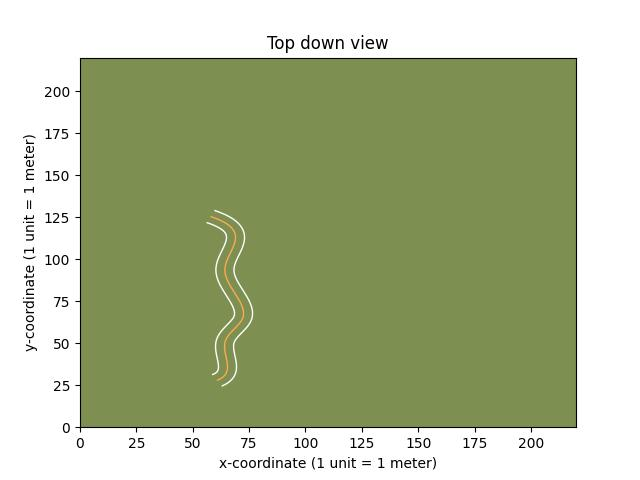
\includegraphics[width=0.5\linewidth]{images/road.jpg}
    \caption{Bird's-Eye View of a road}
    \label{road}
\end{figure}

\begin{figure}[!h]
    \centering
    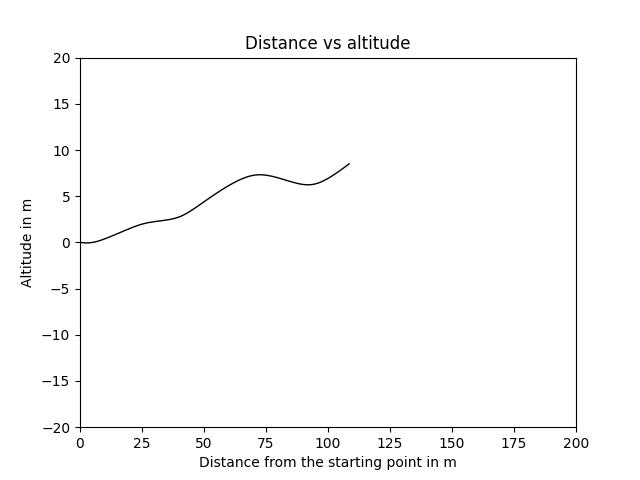
\includegraphics[width=0.5\linewidth]{images/height.jpg}
    \caption{Distance against Height}
    \label{height}
\end{figure}

